%Import de herramientas predefinidas
\documentclass[a4paper,11pt]{scrarticle}
\usepackage[left=2.5cm, right=2.5cm, top=2.5cm, bottom=2.5cm]{geometry}
\usepackage{graphicx}
\usepackage{hyperref}
\usepackage{xcolor}
\usepackage{listings}

\usepackage[style=ieee, backend=biber]{biblatex}
\addbibresource{bib.bib}
%---------------PREAMBULO----------------->
\usepackage{verbatim} %Paquete para comentarios multilínea
\usepackage{graphicx} %Paquete para usar imagenes
\usepackage{amsmath} %Paquete para fuentes y \text
%\usepackage[spanish]{babel}

%<<<<<<<<<<<<<<<<<<<<<<<<<<<<<<<<<<<<<<<<<<<

%---------------SECTION----------------->
%<<<<<<<<<<<<<<<<<<<<<<<<<<<<<<<<<<<<<<<<<<<

\begin{document}
    %---------------COVER PAGE----------------->
    %Entorno para portadas

%---------------README----------------->
%USE \include{Portada} %for import front page from main.tex
%USE \usepackage{amsmath} en el preambulo del main
%<<<<<<<<<<<<<<<<<<<<<<<<<<<<<<<<<<<<<<<<<<<

\begin{titlepage}

%--------------- COMANDO LINEA----------------->
\newcommand{\linea}{\rule{\linewidth}{0.7mm}}                 
\center
%<<<<<<<<<<<<<<<<<<<<<<<<<<<<<<<<<<<<<<<<<<<

%Add logos

\includegraphics[width=0.8\textwidth]{logos.png}\\[0.02cm]
\vfill

%---------------TÍTULO----------------->
\linea
\vfill
\textbf{\Large Compilers: FLEX}\\[0.2cm]
\textbf{\Large }\\[0.2cm]
\linea \\
\vfill
%Title of the Research
\textbf{\large Alumnos:}\\
%<<<<<<<<<<<<<<<<<<<<<<<<<<<<<<<<<<<<<<<<<<<

%Team
    \vfill
    \textbf{\large  \textbf{Álvarez López Carlos Manuel }}\\
    \textbf{\large  \textbf{Hernández Gallardo Daniel Alonso }}\\
    \textbf{\large  \textbf{Jimenez Ortíz Sebastián }}\\
    \textbf{\large  \textbf{López Flores Isaac}}\\
    \vfill
\textbf{Número de equipo: 9}\\ 

%ING. ALBERTO RAFAEL GONZALEZ GARCIA
%Profesor y Grupo
    \textit{\small Profesor:}\\
    \textbf{Rene Adrián Dávila Pérez}\\
    \textit{\small *Grupo 5, Semestre 2025-2*}
    \vfill

%Fecha or Date
    {\large Fecha de entrega: \\ 27 de febrero de 2025}\\
    \newpage
    \end{titlepage} %for import front page
    \newpage
    \tableofcontents
    \newpage

    \section{Objectives}
    This report aims to analyze and demonstrate the functionality of FLEX as a lexical analyzer generator. Two different implementations detecting specific patterns in text strings are presented. The objectives are:
    \begin{itemize}
        \item Understand the operation of FLEX in generating lexical analyzers.
        \item Implement rules for recognizing different patterns in input text.
        \item Analyze the obtained results and their applicability in practical contexts.
    \end{itemize}

        \section{Introduction}
    FLEX is a lexical analyzer generator that processes input text based on defined patterns and generates C code for scanning input streams. This report presents two different lexical analyzers implemented using FLEX. The first analyzer detects digits, non-uppercase characters, and specific patterns of the letter 'a'. The second analyzer identifies email addresses, hexadecimal numbers, and arithmetic operators.

    \section{Theoretical Framework}
    FLEX is a tool for generating scanners. A scanner is a program which recognizes lexical patterns in text. The flex program reads the given input files, or its standard input if no file names are given, for a description of a scanner to generate. The description is in the form of pairs of regular expressions and C code, called rules. FLEX generates as output a C source file, lex.yy.c by default, which defines a routine yylex(). This file can be compiled and linked with the flex runtime library to produce an executable. When the executable is run, it analyzes its input for occurrences of the regular expressions. Whenever it finds one, it executes the corresponding C code.
    \cite{flex_manual}

    \section{Development}
    For the implementation of lexical analyzers, FLEX was used with the following pattern rules:
    \begin{itemize}
        \item \textbf{[0-9]}: Matches any digit from 0 to 9. The classic regular expression, a pattern that already exists and can be found it at \cite{flex_manual}.
        \item \textbf{[\textasciicircum A-Z]}: Matches any character except uppercase letters. The symbol \textasciicircum represents the negation, so the lexer interprets it as non-uppercase letters but allows any other character
        \item \textbf{a\{2,3\}}: Matches exactly two or three occurrences of the letter 'a'. It's simple: the letter 'a' represents what we want the lexer to match, and '{2,3}' establishes a range; it means from 2 to 3 'a's.
        \item \textbf{[A-Za-z0-9.\_\%+-]+@[A-Za-z0-9.-]+.[A-Za-z]\{2,4\}}: Matches email addresses. This regular expression matches email addresses. The pattern before the @ symbol allows any combination of letters (both uppercase and lowercase), numbers, periods (.), underscores (\_), percentage symbols (\%), plus signs (+), and hyphens (-). After the @ symbol, it allows letters, numbers, and periods, and finally, the domain must have a 2-4 letter extension (such as ".com" or ".info").
        \item \textbf{0x[0-9A-Fa-f]+}: Matches hexadecimal numbers.This regular expression matches hexadecimal numbers. The 0x prefix indicates that the number is hexadecimal. Then, the pattern [0-9A-Fa-f]+ allows one or more digits that can be numbers (0-9) or letters from A to F, in either uppercase or lowercase.
        \item \textbf{[+\textbackslash -*/\%]}: Matches arithmetic operators. This regular expression matches arithmetic operators. The character set [+\textbackslash -*/\%] allows any of the following symbols: plus (+), minus (-), multiplication (*), division (/), and modulo (%).
    \end{itemize}
    The lexer reads the input character by character, attempting to match these patterns. When a match is found, the corresponding action (e.g.printing the recognized token) is executed. If multiple patterns match, FLEX prioritizes the longest match (for trailing context rules, this includes the length of the trailing part, even though it will then be returned to the input) or the first rule defined in case of equal length.\\
    Two separate FLEX files were created to process these patterns and generate the corresponding lexical analyzer.

    \subsection{First Implementation}
    This implementation focuses on detecting fundamental character classes in text, including:
    \begin{itemize}
        \item Sequences of two or three 'a' characters.
        \item Non-uppercase letters.
        \item Digits (0-9).
    \end{itemize}
    The goal is to filter and classify simple textual patterns that may appear in programming.

    \subsection{Second Implementation}
    This implementation enhances the complexity of recognition by detecting structured text patterns such as:
    \begin{itemize}
        \item Email addresses.
        \item Hexadecimal numbers.
        \item Arithmetic operators.
    \end{itemize}
    These patterns are commonly found in programming languages and data validation tasks, which is valuable to identify when are we talking about building a compiler.
    \newpage
    \section{Results}
    Below are examples of input and output obtained from the execution of the analyzers:
    \subsection{First Implementation}
    \begin{figure}[h]
        \centering
        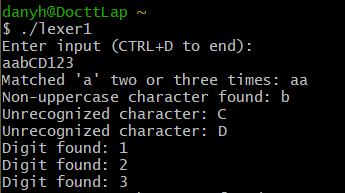
\includegraphics[width=0.75\linewidth]{R1.png}
        \caption{Evidence N1.}
    \end{figure}
    \begin{verbatim}
    Input: aabCD123
    Output:
    Matched 'a' two or three times: aa
    Non-uppercase character found: b
    Unrecognized character: C
    Unrecognized character: D
    Digit found: 1
    Digit found: 2
    Digit found: 3
    \end{verbatim}
    The output correctly categorizes each character group according to the predefined rules, proving that the lexer can accurately process mixed input types.

    \subsection{Second Implementation}
    \begin{figure}[h]
        \centering
        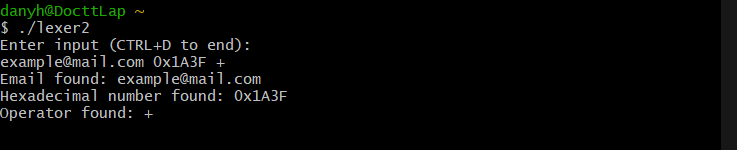
\includegraphics[width=0.75\linewidth]{R2.png}
        \caption{Evidence N2.}
    \end{figure}
    \begin{verbatim}
    Input: example@mail.com 0x1A3F +
    Output:
    Email found: example@mail.com
    Hexadecimal number found: 0x1A3F
    Operator found: +
    \end{verbatim}
    This implementation successfully recognized structured text elements such as email addresses, hexadecimal numbers, and arithmetic operators, validating its practical applicability.
    \section{Conclusion}
    We can truly state that the objectives were completely accomplished because we understand how FLEX works as a lexical analyzer generator. We implemented rules for recognizing different patterns in input text, using knowledge of how FLEX works and how it uses regular expressions to identify the tokens.
    Also, we obtained and analyzed the results provided by the patterns that we used, seeing their applicability in practical contexts. This is an important point because now we can clearly see FLEX as an important part to understant more complicated tools in order to build our future compiler and view it beyond the theoretical aspects.
    \nocite{*}
    \printbibliography
    
\end{document}



    %<<<<<<<<<<<<<<<<<<<<<<<<<<<<<<<<<<<<<<<<<<<
   
\end{document}